\section{\textbf{Metodolog\'ia}}
\subsection{Dise\~no de Experimentos}
Para describir el planeamiento pre-experimental para el dise\~no de experimentos de este trabajo (con la informaci\'on disponible hasta el momento) se usan los \textit{lineamientos} desarrollados en el libro de \textit{Douglas C. Montgomer}y \cite{montgomeryx}. El esquema del procedimiento recomendado en los lineamientos para el desarrollo de esta etapa, incluye lo siguiente:
\begin{itemize}
\item [1.] \textbf{Reconocimiento y definici\'on del problema:} consiste en desarrollar una declaraci\'on clara y sencilla del problema. Una clara definici\'on del problema, normalmente contribuye substancialmente a una mejor comprensi\'on del fen\'omeno que est\'a siendo estudiado y a la soluci\'on final de dicho problema.
\item [2.] \textbf{Selecci\'on de factores, niveles y rangos:} consiste en enumerar todos los posibles factores que pueden influenciar el experimento. Incluye tanto los factores de dise\~no potencial (los que potencialmente se podr\'ian querer modificar en los experimentos) y los factores perturbadores (los que no se quieren estudiar en el contexto del experimento). Tambi\'en, se deben seleccionar los rangos sobre los que var\'ian los distintos factores y los niveles espec\'ificos sobre los que se aplicar\'an las iteraciones del experimento.
\item [3.] \textbf{Selecci\'on de la variable de respuesta:} debe proveer informaci\'on \'util sobre el fen\'omeno que est\'a siendo estudiado.
\item [4] \textbf{Selecci\'on del dise\~no de experimental:} se refiere a aspectos claves del experimento tales como el tama\~no de la muestra, la selecci\'on del orden adecuado para la ejecuci\'on de los intentos experimentales y la decisi\'on de bloquear o no algunas de las restriciones de aleatoriedad en la pruebas.
\item [5] \textbf{Llevar a cabo el experimiento:} en esta etapa, es de vital importancia, monitorear el proceso cuidadosamente para asegurar la correcta ejecuci\'on del expe\-rimento con respecto a lo planeado.
\end{itemize}
\subsubsection{Declaraci\'on del Problema}
Estudiar el comportamiento de \textit{Cubic Spline Interpolation} como medida de distancia utilizada en el descubrimiento de reglas significativas en series temporales complejas y en presencia de ruido.\par
\textit{Cubic Spline Interpolation} y otras medidas medidas de distancia ser\'an incorporadas en dos los algoritmos espec\'ificos llamados \textit{\textbf{\enquote{Rule Bit Saves}}} y \textit{\textbf{\enquote{Find Antecedent Candidates}}} propuestos por Mohammad Shokoohi-Yekta y colaboradores en \cite{main}. Es importante se\~nalar, que por cada medida de distancia utilizada, se crear\'a una nueva versi\'on de ambos algoritmos.\par
La precisi\'on en el hallazgo de reglas significativas ser\'a medido a trav\'es de la ejecuci\'on, la comparaci\'on y el an\'alisis de cada versi\'on de los algoritmos, mediante la utilizaci\'on de al menos cinco fuentes de datos temporales de complejidad variada y en presencia de diferentes grados de ruido.
\subsubsection{Factores}
En el dise\~no de experimentos, un factor es aquel componente que tiene cierta
influencia en las variables de respuesta \cite{montgomeryx}. El objetivo de un experimento es determinar esta influencia. A su vez, cada factor cuenta con varios niveles posibles con los cuales experimentar.\par
Usando la informaci\'on recolectada en esta etapa de la investigaci\'on, as\'i como la experiencia adquirida por el estudiante y expuesta en los cap\'itulos anteriores, se han seleccionado inicialmente los siguientes dos factores para su estudio:
\begin{itemize}
\item [1.] \textbf{Las m\'etricas o medidas de distancia}\\
Se utilizar\'an dos algoritmos para la ejecuci\'on del dise\~no de experimental:\\
1- \textit{\textbf{\enquote{Rule Bit Saves}}} utilizado en la identificaci\'on de potenciales reglas o patrones significativos (\textit{\textit{detecci\'on de reglas \textit{Motif en \cite{main}}}}) y 2- \textit{\textbf{\enquote{Find Antecedent Candidates}}}, creado para probar capacidad predictiva de las reglas motif identificadas en el algoritmo anterior, sobre cada uno de los conjuntos de datos. Ambos algoritmos ser\'an moficados y adaptados a cada medida de distancia y su ejecuci\'on sobre cada conjunto de datos, ser\'a realizada en forma controlada e independiente.\par
Las medidas de distancia utilizadas, son las siguientes:
\begin{itemize}
\item \textbf{\textit{Distancia Euclidiana}}
\item \textbf{\textit{Swale}}
\item \textbf{\textit{Spade}}
\item \textbf{\textit{EPR}}
\item \textbf{\textit{Cubic Spline Interpolation}}
\end{itemize}
\item [2.] \textbf{El conjunto de datos, tama\~no y complejidad}\\
Los niveles de ruido, la valoraci\'on de la complejidad y el tama\~no de cada conjunto de datos, se encuentran a\'un pendientes de determinar. Dicha clasificac\'ion estar\'a dada en al menos tres niveles que permitan medir la complejidad de cada conjunto de datos.\\
En el experimento, se utilizar\'an los siguientes conjuntos de datos:
\begin{itemize}
\item 1. \textbf{\enquote{Energy disaggregation dataset}:} contiene el amperaje del consumo diaro de una casa promedio durante un a\~no.
\item 2. \textbf{\enquote{Zebra finch vocalizations}:} contiene las grabaciones del canto de un p\'ajaro \textit{\enquote{Zebra}} durante sus primeros 100 d\'as de vida.
\item 3. \textbf{\enquote{Daily basis activity data set}:} este conjunto de datos contiene informaci\'on telem\'etrica de actividades cotidianas de una persona.
\item 4. \textbf{\enquote{NASA telemetry data}:} contiene medidas de voltajes err\'oneas producidas por las v\'alvulas utilizadas en los transbordadores espaciales de la NASA, utilizadas para el estudio y la detecci\'on de anomal\'ias .
\end{itemize}
\end{itemize}
Los conjuntos de datos anteriores, fueron seleccionados pensando primordialmente en facilitar la ejecuci\'on del dise\~no de experimentos con base en los resultados obtenidos en \cite{main}. Lo anterior permitir\'a generar resultados mucho m\'as confiables durante la ejecuci\'on de las pruebas.\par
En la tabla 1, presentada a continuaci\'on, se resumen los factores que se utilizar\'an para evaluar los resultados de ambos algoritmos, para cada conjunto de datos.
\begin{center}
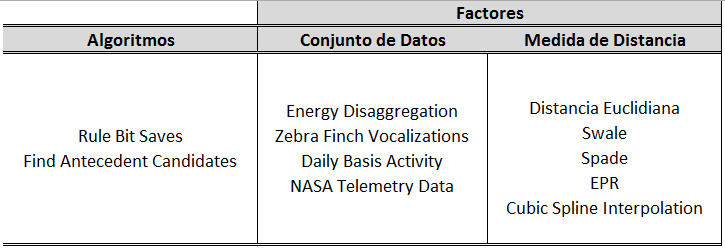
\includegraphics[scale=0.7]{factors.png}\\
\vspace*{10pt}
\footnotesize{\textbf{Tabla 1.} Resumen de los factores que se utilizar\'an en el dise\~no de experimentos.}
\end{center}
\subsubsection{Variables de Respuesta}
Dado que la hip\'otesis afirma maximizar el nivel de exactitud en la identificaci\'on de reglas significativas y el hallazgo de segmentos antecedentes sobre los diferentes conjuntos de datos, se ha seleccionado \textit{\textbf{la exactitud}} como la \'unica variable de respuesta para ambos algoritmos:
\begin{itemize}
\item [1.] \textbf{\textit{Medici\'on de la exactitud sobre el algoritmo \enquote{Rule Bit Saves}}}\\
C\'alculo del total de aciertos en la identificaci\'on de reglas \textit{motif} (potenciales reglas significativas) sobre cada conjunto de prueba, mediante la ejecuci\'on de las cinco diferentes versiones del algoritmo.
\item [2.] \textit{\textbf{Medici\'on de la exactitud sobre \enquote{Find Antecedent Candidates}}}\\ 
Una vez que las reglas motif han sido identificadas, se requiere calcular para cada una de ellas, el total de aciertos en el hallazgo de segmentos antecedentes (\textit{predicciones}), sobre cada conjunto de datos, para cada una de las medidas de distancia implementadas en las cinco versiones del algoritmo.
\end{itemize}
\subsubsection{Recolecci\'on de Datos}
Las variables de respuesta ser\'an recolectadas de forma autom\'atica, una vez concluida la ejecuci\'on de cada una de las versiones de ambos algoritmos.\\
La automatizaci\'on de la recolecci\'on de las variables de respuesta ser\'a posible mediante la implementaci\'on del ambiente de pruebas.
\subsubsection{An\'alisis Estad\'istico}
Una vez conclu\'ida la ejecuci\'on del experimento, se deben analizar los resultados para comparar ambos algoritmos en sus diferentes versiones. Para esta comparaci\'on, se debe analizar si existe una diferencia significativa en los promedios obtenidos de la variable de respuesta para cada uno de los distintos grupos.
Un an\'alisis de varianza permite saber si la diferencia en la media de varias poblaciones es significativa debido a la influencia de alguno de los factores \cite{designexp}.\par 
En primera instancia, se har\'an las pruebas de normalidad utilizando el valor \textit{p} para mostrar si los resultados cumplen o no los requisitos para una prueba param\'etrica. Posteriormente, una vez realizada la prueba de normalidad, se utilizar\'a el m\'etodo estad\'istico, no param\'etrico llamado \textit{\textbf{\enquote{Kruskal-Wallis-Test}}}. Mediante el uso de este m\'etodo, no se tiene que asumir que las poblaciones siguen una distribuci\'on normal, \'unicamente se utilizar\'an muestras independientes provenientes de distintas fuentes de datos; poblaciones no relacionadas cuyas muestras no se afectan unas con otras \cite{kruskwal}.
\subsection{Ambiente de Desarrollo}
Para el desarrollo de la propuesta de investigaci\'on actual, se implementar\'a una plataforma que cumpla con dos caracter\'isticas principales:
\begin{itemize}
\item [1.] Que la plataforma se pueda ejecutar sobre los sistemas operativos Windows y Linux: esto implica que el c\'odigo fuente debe ser escrito en un lenguaje de programaci\'on capaz de correr en los dos sistemas operativos, con un n\'umero m\'inimo de cambios y que las bibliotecas utilizadas est\'en disponibles para los dos sistemas operativos.
\item [2.] Que las herramientas y bibliotecas a utilizar sean gratuitas al menos para uso acad\'emico.
\end{itemize}
Basado en estas dos caracter\'isticas, se ha elegido una lista de posibles soluciones de software a utilizar. Como se indica, esta lista es preliminar, por lo que se preveen posibles cambios durante el desarrollo de la tesis.
\begin{itemize}
\item \textbf{Sistema Operativo:} Windows 8.1 y Linux Ubuntu 16.04.1 LTS.
\item \textbf{Lenguaje de programaci\'on:} Matrix Laboratory (MATLAB).
\end{itemize}
